In this section, we apply the BriefCASE tool to the development of a UAV surveillance system in which a UAV receives commands from a ground station to conduct surveillance along a geographical feature such as a river. The on-board mission computer then generates a flight plan consisting of a series of waypoints that the UAV must traverse to complete its mission. The UAV is also given a set of \textit{keep-in} and \textit{keep-out} zones that may constrain its flight path.

We have modeled the system architecture of the UAV in AADL.  It includes a Mission Computer for communicating with the ground station and generating flight plans, and a Flight Control Computer for UAV navigation.  The Mission Computer architecture model includes hardware components such as a processor, memory, and communication devices, as well as software.
%
The initial software architecture model (shown in Figure~\ref{fig:sw-initial}) contains drivers for communication with the Ground Station and Flight Control Computer, a Waypoint Manager component that provides flight plan coordinates to the Flight Control Computer, and the Flight Planner.  The Flight Planner is the open-source UxAS software developed by AFRL~\cite{uxas}. For this application, UxAS accepts three types of messages.  The \textit{Operating Region} message defines where the UAV can and cannot fly.  The \textit{Line Search Task} message contains a series of waypoints that the UAV should traverse.  The waypoints typically lie along some geographical feature of interest, such as a river or railway.  Note that the UAV may not be able to directly traverse the Line Search Task waypoints due to no-fly zone constraints specified in the Operating Region message.  Anytime after receiving the Operating Region and Line Search Task messages, a ground station can transmit an \textit{Automation Request} message, which instructs UxAS to generate a flight plan that satisfies these constraints.  UxAS passes the flight plan in an \textit{Automation Response} message to the Waypoint Manager.  Because the Flight Control Computer can only process a small number of waypoints at a time, the Waypoint Manager parcels a small number of waypoints corresponding to the current UAV position, and sends them to the Flight Control Computer over a serial connection via the UART Driver.

\begin{figure}[h]
	\centering
	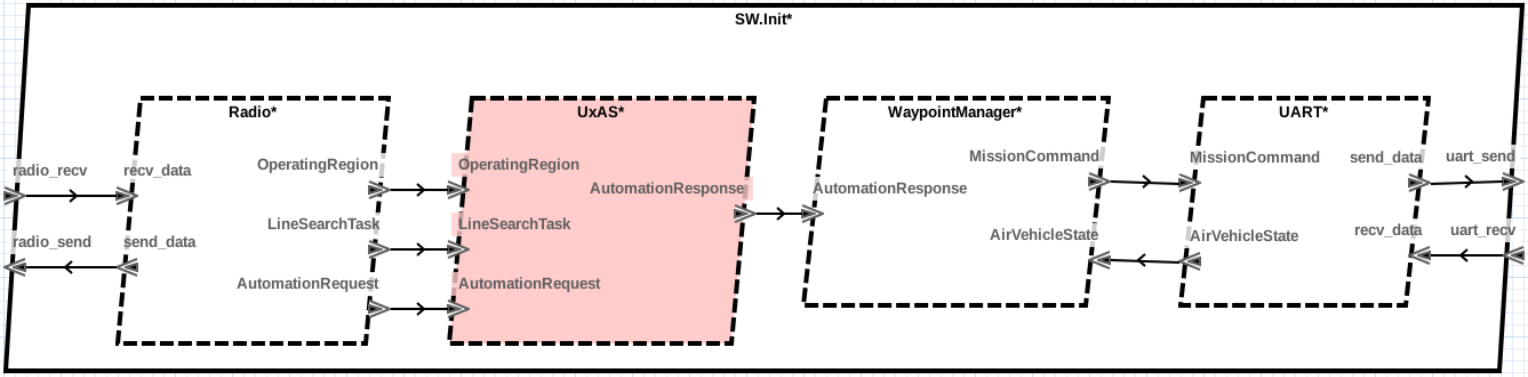
\includegraphics[width=1\columnwidth]{figs/sw-initial.png}
	\caption{Initial software architecture.} 
	\label{fig:sw-initial} 
\end{figure}

Within the software model, we have formalized some of the high-level requirements as assume-guarantee contracts.  We perform a formal analysis using the AGREE tool (which is integrated with the BriefCASE environment) to verify that the model satisfies the contracts.  For the initial version of our design, the verification passes.
%
Although we are satisfied with the results of the formal verification using AGREE, we have not yet analyzed the design for cyber-vulnerabilities.  
In BriefCASE, we analyze the model using one (or more) of the integrated cybersecurity analysis tools.  The tools generate a list of new requirements corresponding to cyber vulnerabilities found in the design.  To satisfy these requirements we need to mitigate the vulnerabilities discovered by the analysis by modifying the design.
%
For example, because we annotated the open-source UxAS component as \texttt{uncontrolled} (colored red in Figure~\ref{fig:sw-initial}), the cyber analysis tools generate requirements for ensuring unverified or malicious code (that could potentially be included in the component) will not impact other processes. 

In total, eight cyber requirements are generated and imported into our model.  These include one \textit{sandboxing} requirement, four \textit{well-formedness} requirements, two requirements for \textit{monitoring} the behavior of the open-source UxAS component, and an \textit{attestation} requirement for ensuring the ground station software has not been tampered with.  Requirements are imported into the model as goals in a Resolute assurance case.  Because we can run Resolute at any time during development, we can easily determine for a given snapshot of the model which requirements are not yet supported by evidence.

The intent of the \textit{well-formedness} requirements is to prevent malformed messages from causing a buffer overrun or code injection attack.  In the UAV design, such messages are most likely to originate from a remote source or the uncontrolled UxAS component.  By placing filters on the connections upstream of mission-critical components, such attacks could be mitigated.  The Filter transform is therefore applied for each well-formedness requirement, inserting filter components on the incoming and outgoing UxAS connections.  

The filter behavior for each component is specified in AGREE.  Not only does this enable formal verification within the modeling environment, but it also provides a means for synthesizing the component implementation in a provably correct manner using the SPLAT tool.  Because SPLAT is integrated with BriefCASE, the proof it emits when synthesizing component code is used as evidence in the Resolute goal for the corresponding mitigation.  When Resolute evaluates whether such a goal is supported by evidence, it checks for the existence of the synthesis proof in addition to verifying the architecture is correct.  

The AGREE filter policies for the four UxAS connections are similar, and check that record values contained in the messages are within appropriate ranges.  For example, the Automation Response message filter, which drops message containing malformed flight plans, is defined as shown in Figure~\ref{fig:automation-response-filter}.  Although Latitude, Longitude and Altitude are defined as 64-bit \textit{reals}, the filter ensures only messages containing waypoint values between (-90,90), (-180,180), and (0,15000), respectively. 

\begin{figure}[h]
	\centering
	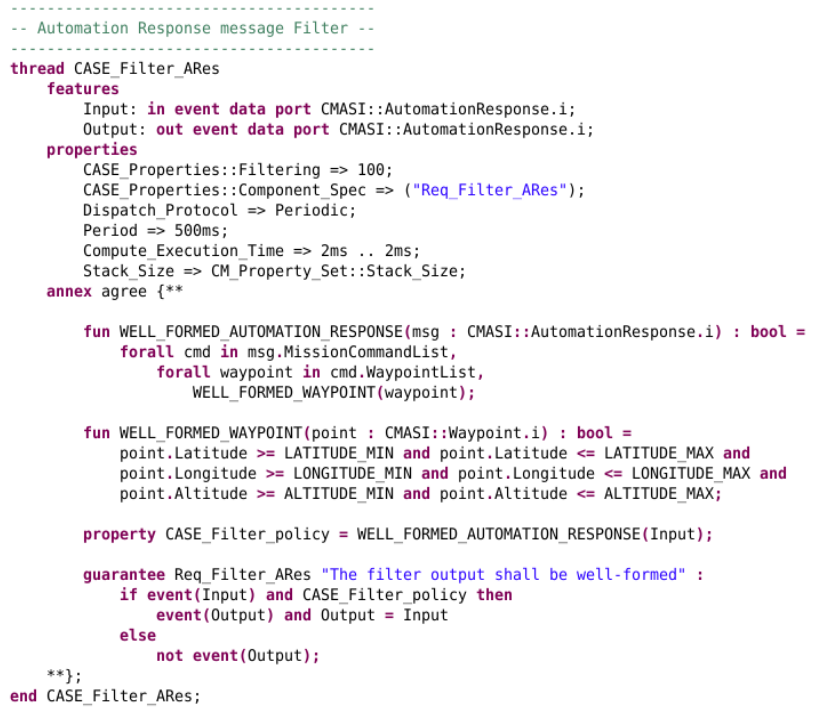
\includegraphics[width=1\columnwidth]{figs/automation-response-filter.png}
	\caption{Automation Response Filter specification.} 
	\label{fig:automation-response-filter} 
\end{figure}

In addition to monitoring the UxAS output for malformed messages, we must also monitor for suspicious behavior.  This requires adding components for detecting that UxAS has crashed, as well as monitoring the correctness of the flight plans it produces.  The Monitor transform is applied for this class of mitigation.  In general, monitors observe a channel and compare its contents against a reference signal or constant.  The monitor policy specifies acceptable comparisons, and if violated, the monitor sends out an alert.  A monitor can choose to \textit{gate} the observed signal, in which case it also acts as a special kind of filter and drops the message if the policy is violated.  The \textit{monitoring} requirements drive two transforms.  The first adds a \textit{response} monitor to send an alert if UxAS does not emit a response within a set amount of time from receiving a request.  The second adds a \textit{geofence} monitor to ensure that generated flight plans are compliant with the specified keep-in and keep-out zones.  The Geofence Monitor is a gated monitor; it prevents the observed Automation Response message from reaching the Waypoint Manager. 

Similar to the filters, the monitor policies are specified in AGREE. The Response Monitor specification is shown in Figure~\ref{fig:response-monitor}, and the Geofence Monitor specification is shown in Figure\ref{fig:geofence-monitor}. 

\begin{figure}[h]
	\centering
	\includegraphics[width=1\columnwidth]{figs/response-monitor.png}
	\caption{Response Monitor specification.} 
	\label{fig:response-monitor} 
\end{figure}

\begin{figure}[h]
	\centering
	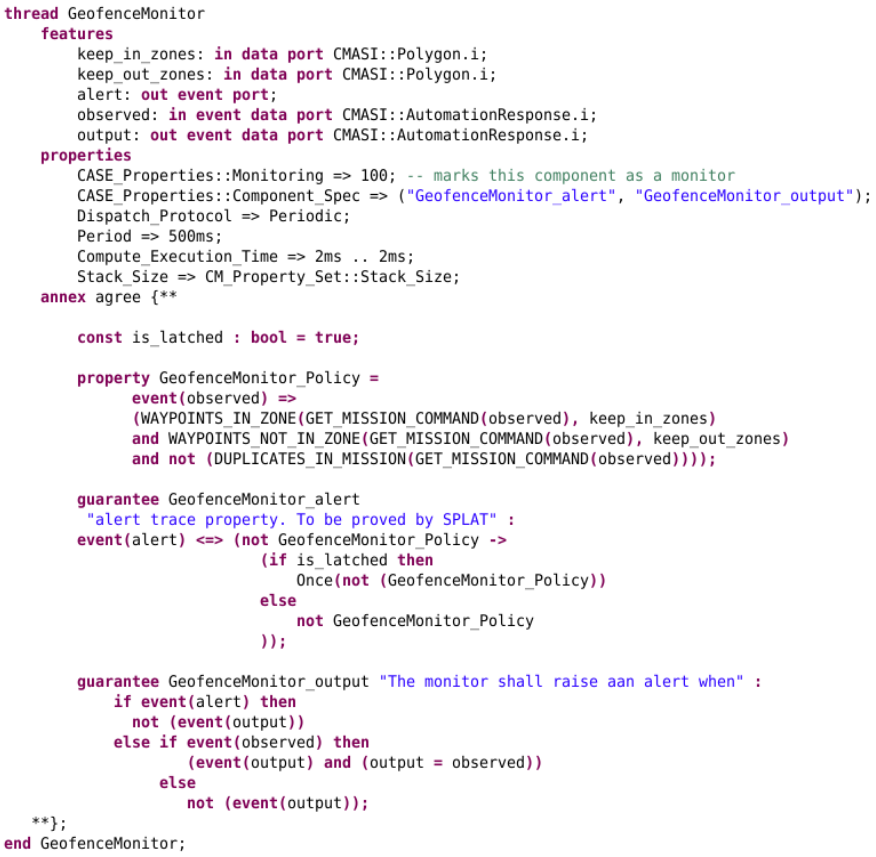
\includegraphics[width=1\columnwidth]{figs/geofence-monitor.png}
	\caption{Geofence Monitor specification.} 
	\label{fig:geofence-monitor} 
\end{figure}

% Describe attestation?

After transforming the model to address the cyber requirements, the software architecture now appears as shown in Figure~\ref{fig:hardened-sw}.  The components in green were added to the model by way of an automated BriefCASE transform and are critical for mitigating cyber attacks. 
We formally verify the model with AGREE to show that all of the component contracts are satisfied, including the new contracts introduced during the model transformations.
Because it is imperative that these high-assurance component implementations are correct,
we run the SPLAT tool to produce provably-correct code.  
The synthesized code is output to a directory in the build file system with the location specified for each component in the model.  The corresponding correctness proof is used in our assurance case as additional evidence that the vulnerability has been properly mitigated.

\begin{figure*}[h]
	\centering
	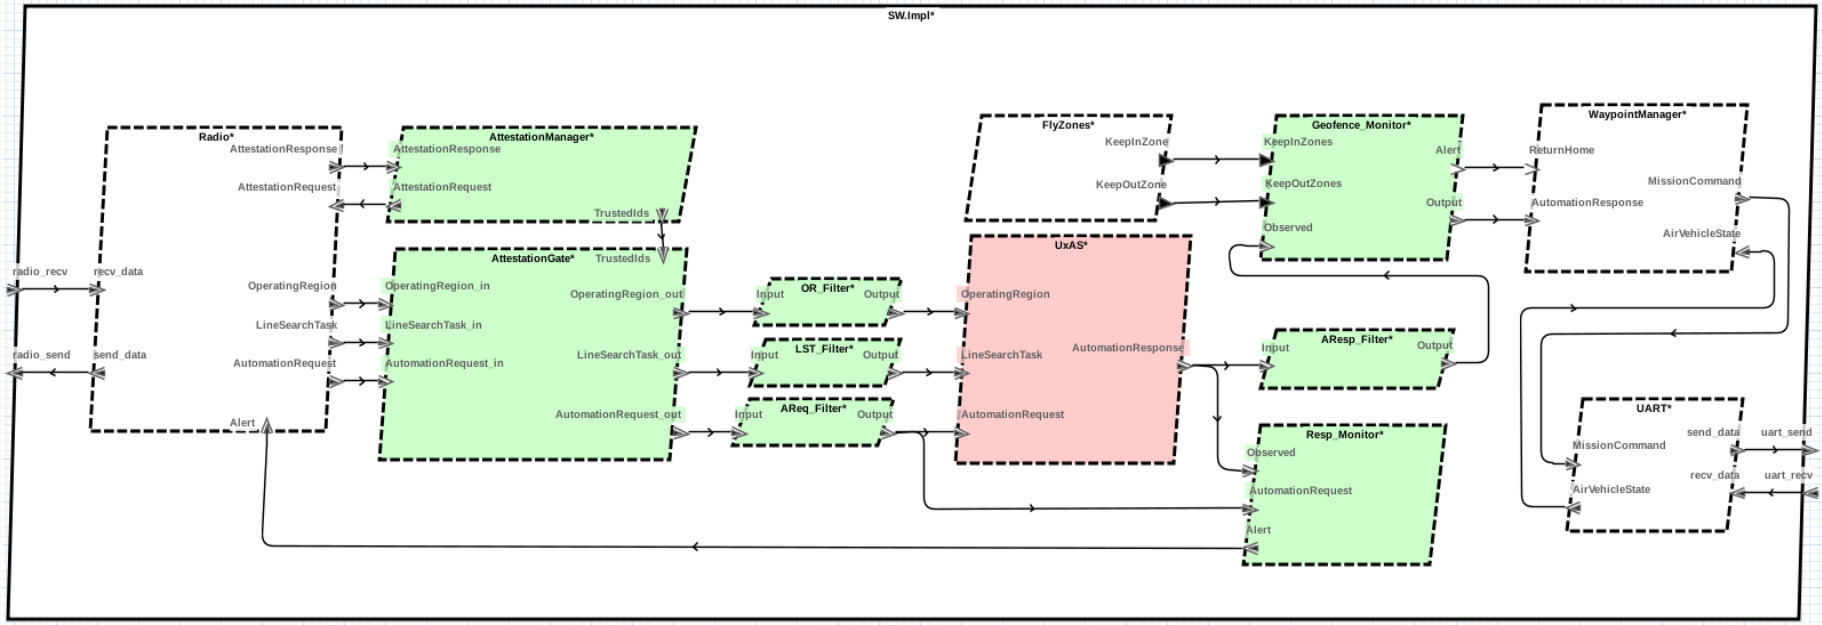
\includegraphics[width=1\columnwidth]{figs/hardened-sw.png}
	\caption{Cyber-resilient software architecture.} 
	\label{fig:hardened-sw} 
\end{figure*}

Once we have determined that the model is correct and satisfies its cyber requirements, and the software components in the model have been implemented, either by SPLAT or other means, the system can be built and deployed.  We run the HAMR tool to generate the component stubs and infrastructure code necessary to enable component communication and execution according to a specified schedule.
HAMR translates the AADL system model to code that implements threading infrastructure and inter-component communication and is consistent with the AADL specification computational model. 

% Something about seL4?